\documentclass[a4paper,11pt,twoside]{article}
% Encoding lokal, da manche Editoren danach schauen
\usepackage[utf8]{inputenc} 
\usepackage{ihr-15}

\title{Benutzerhandbuch „Interaktiver Haushaltsrechner“}
 
\date{Version vom 18. Mai 2015, reformatiert am 1. Juli 2015}

\begin{document}
\maketitle
\tableofcontents
\newpage
\seitezwei
\newpage

\section{Einleitung}
Das vorliegende Benutzerhandbuch soll Ihnen eine leichte Einf\"uhrung in
Aussehen und Bedienung unserer Website vermitteln. Alle M\"oglichkeiten werden
mit Hilfe von Bildern beschrieben.
\section{Registrieren und Anmelden}
Auf jeder verf\"ugbaren Seite befindet sich in der oberen rechten Ecke ein
Registrieren- und ein Login-Link, welcher Sie zu den jeweiligen Seiten
f\"uhrt.
\begin{center}
  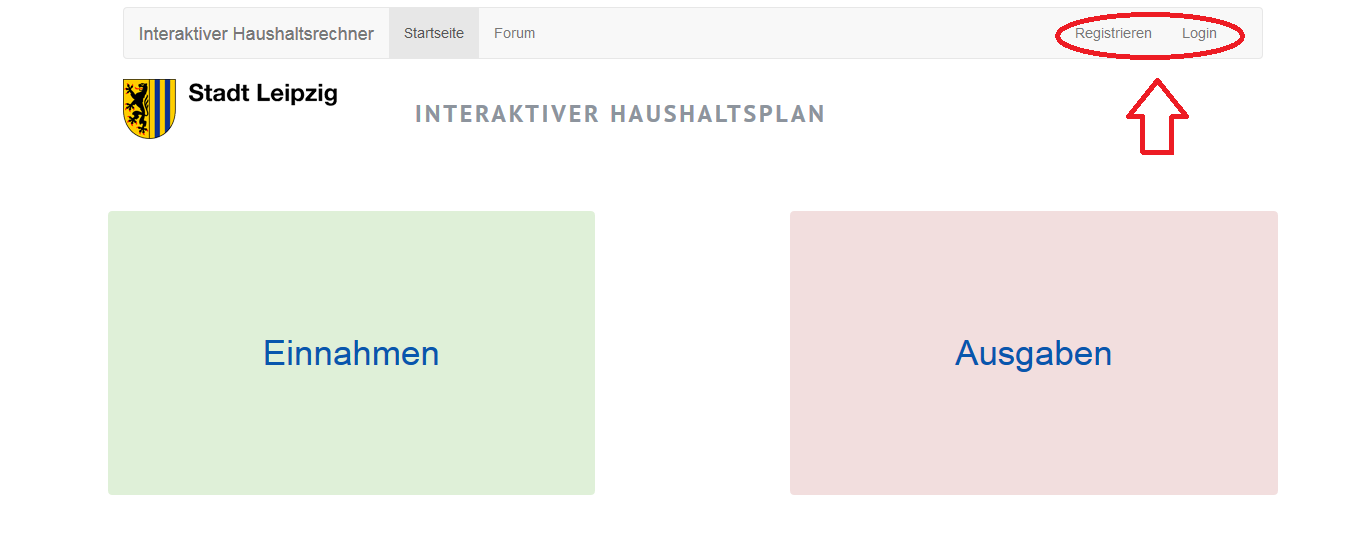
\includegraphics[width=\textwidth]{Bilder/Anmeldung.png}
\end{center}

\subsection{Registrierung}
Nachdem Sie auf Registrieren gedr\"uckt haben, kommen Sie auf die
Registrierungsseite, auf der Sie sich einen Account f\"ur den Haushaltsrechner
Leipzig erstellen.
\begin{center}
  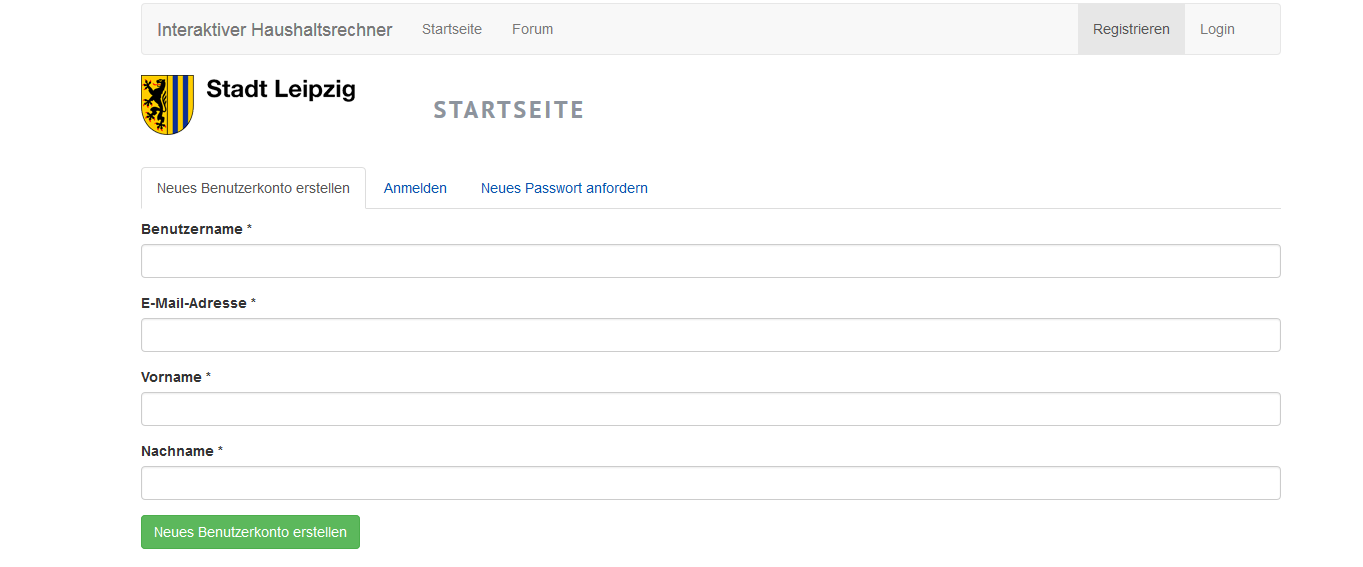
\includegraphics[width=\textwidth]{Bilder/registrierung.png}
\end{center}
Hier m\"ussen Sie nur die Felder mit den entsprechenden Daten ausf\"ullen und
auf "`Neues Benutzerkonto erstellen"' dr\"ucken.
\subsection{Anmeldung}
Sofern Sie schon einen Account besitzen und sich nur Anmelden wollen um das
Forum nutzen zu k\"onnen, m\"ussen Sie auf Login dr\"ucken.
\begin{center}
  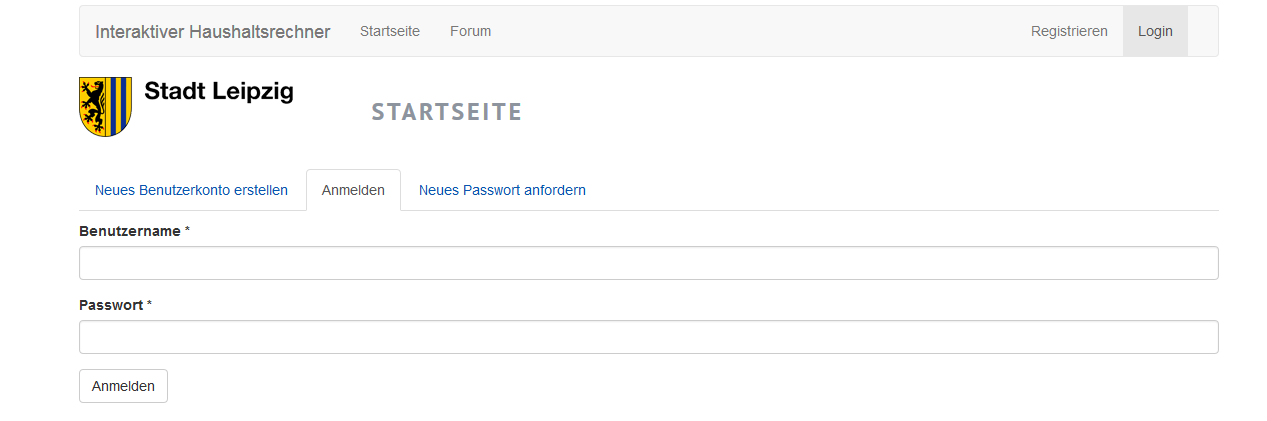
\includegraphics[width=\textwidth]{Bilder/anmelden.png}
\end{center}
Nach der Eingabe Ihres Benutzernamens und Passworts dr\"ucken Sie auf
"`Anmelden"'.
\subsection{Passwort vergessen}
Sofern Sie ihr Passwort vergessen haben, k\"onnen Sie dieses durch Angabe
ihres Benutzernamens oder ihrer Email zur\"ucksetzen. Sie bekommen dann in
einer Email ein neues Passwort zugesendet.  Diese Seite ist erreichbar indem
Sie entweder von der Registrierungsseite oder der Loginseite auf "`Neues
Passwort anfordern"' dr\"ucken.
\begin{center}
  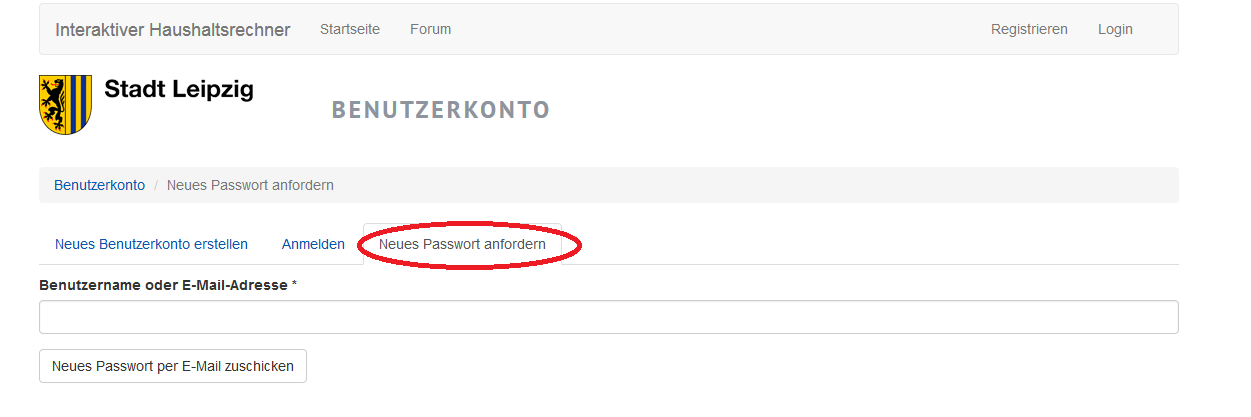
\includegraphics[width=\textwidth]{Bilder/neuesPasswort.png}
\end{center}
\section{Haushaltsplan}
Auf der Hauptseite (auf diese kommen Sie, sofern Sie auf Stadt Leipzig oder
Interaktiver Haushaltsrecher oder Startseite dr\"ucken) k\"onnen Sie sich
zwischen der Ansicht auf die Einnahmen oder die Ausgaben der Stadt Leipzig
entscheiden.
\begin{center}
  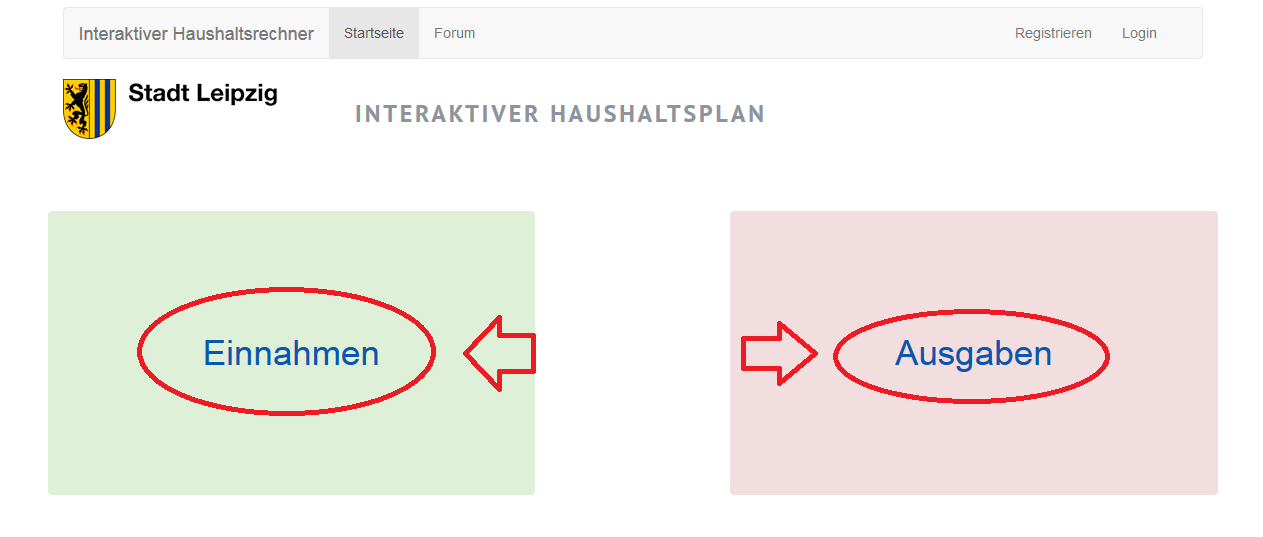
\includegraphics[width=\textwidth]{Bilder/einAus.png}
\end{center}
In diesem Beispiel wurde auf die Einnahmen gedr\"uckt.

\begin{center}
  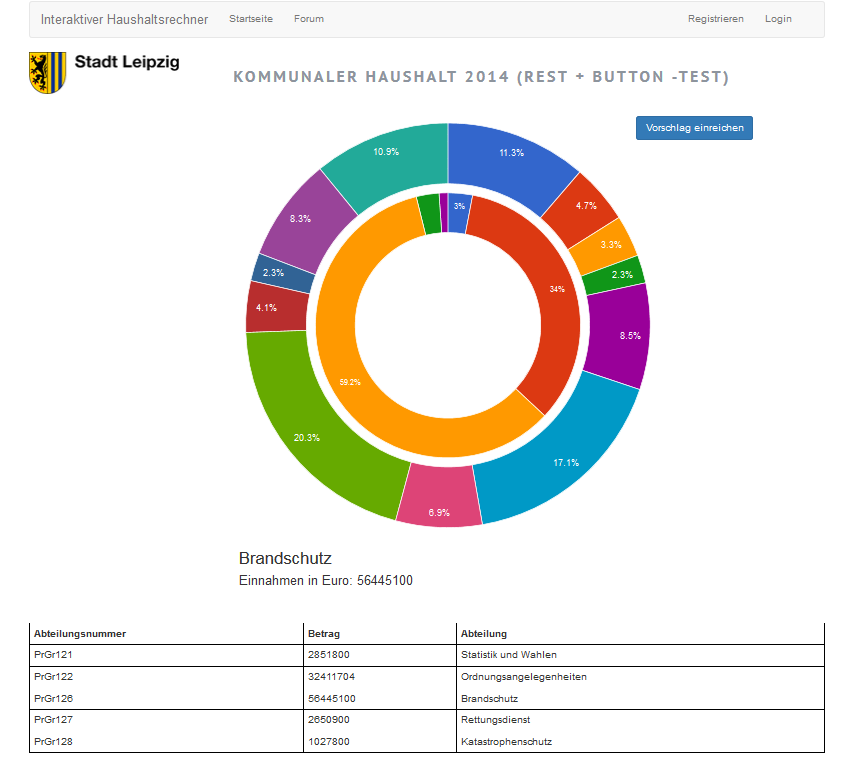
\includegraphics[width=\textwidth]{Bilder/piechart.png}
\end{center}
Hier sehen Sie ein Kreisdiagramm, welches prozentuell die Ausgaben der
verschiedenen Abteilungen der Stadt Leipzig anzeigt.  Indem Sie auf einen
Block dr\"ucken, sehen Sie die darunter liegenden Schichten. Es gibt f\"ur
jeden Bereich drei Unterschichten (also ingesammt vier Kreisdiagramme). Wenn
Sie mit der Maus \"uber einen Bereich im Kreisdiagramm gehen, sehen Sie unter
dem Kreisdiagramm den Abteilungsnamen sowie auch den Geldbetrag. Zu beachten
ist, dass in den meisten F\"allen das letzte Glied des Kreisdiagramms
"`Sonstiges"' ist. Dieses ist nicht klickbar und ist eine Zusammenfassung
aller Bereiche, welcher weniger als 2\% betr\"agt. Diese sind in der Tabelle
einseh- und klickbar.

Unter dem Kreisdiagramm ist eine Tabelle, welche genauere Angaben zum zuletzt
gedr\"ucktem Bereich enth\"alt. Die Tabelle ist genauso wie das Kreisdiagramm
klickbar.

Sofern Sie einen anderen Abteilungsbereich sehen wollen, m\"ussen Sie ihn nur
im Kreisdiagramm anklicken.

Der Vorschlag einreichen Button bringt Sie direkt in den richtigen
Foruenabschnitt, um f\"ur den derzeitig ausgew\"ahlten Bereich einen Vorschlag
zu schreiben.

\section{Forum}
Im Forum k\"onnen f\"ur die einzelnen Produktbereiche Vorschl\"age gelesen,
bewertet, kommentiert und erstellt werden. Desweiteren kann die Stadt selbst
auch Diskussionen starten.

\begin{center}
  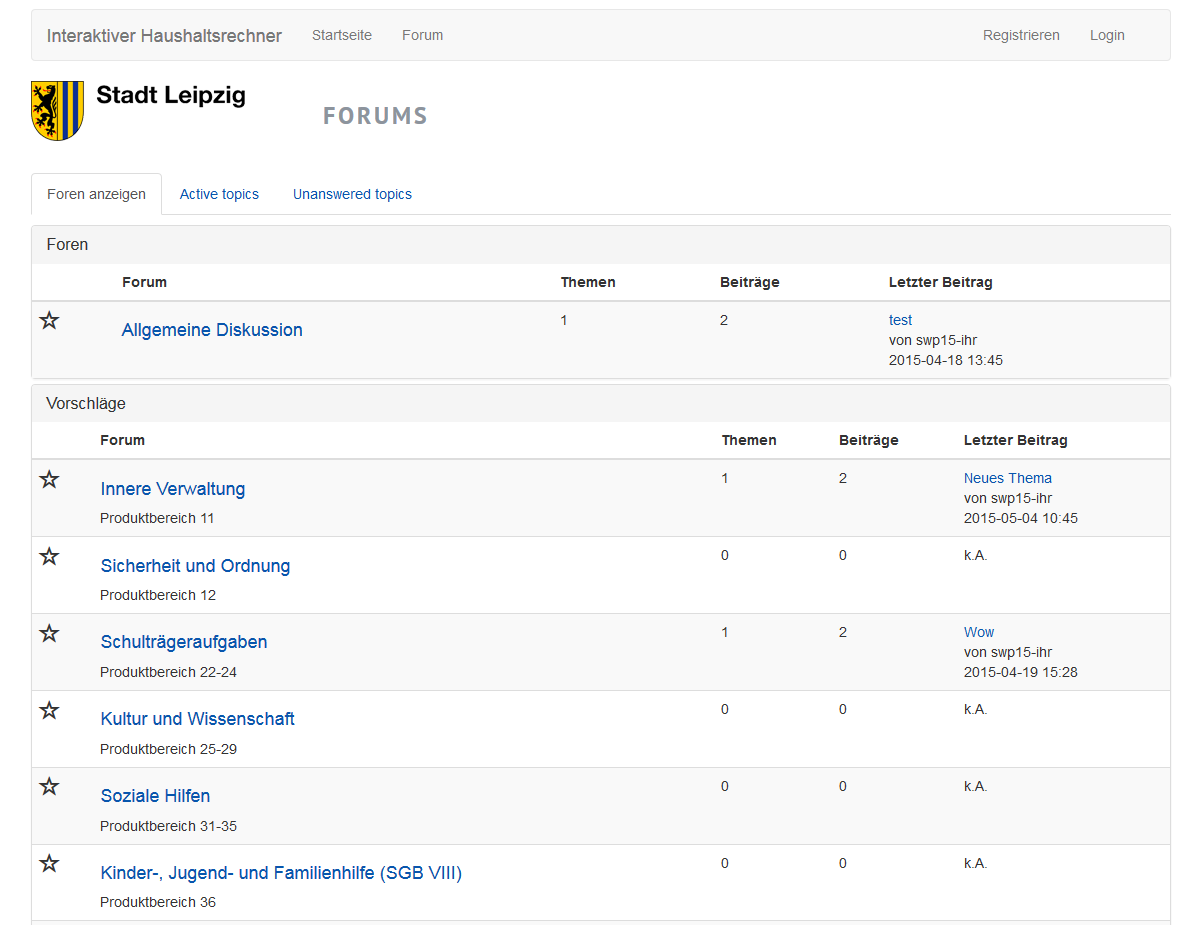
\includegraphics[width=\textwidth]{Bilder/forum.png}
\end{center}
Um das Forum anzuschauen ist keine Anmeldung notwendig, f\"ur alles weitere
ist sie es jedoch.
\subsection{Vorschlag erstellen}
Ein neues Thema erstellen Sie, indem Sie auf einen Bereich klicken (in diesem
Beispiel Kultur und Wissenschaft) und auf Forenthema hinzuf\"ugen dr\"ucken.

\begin{center}
  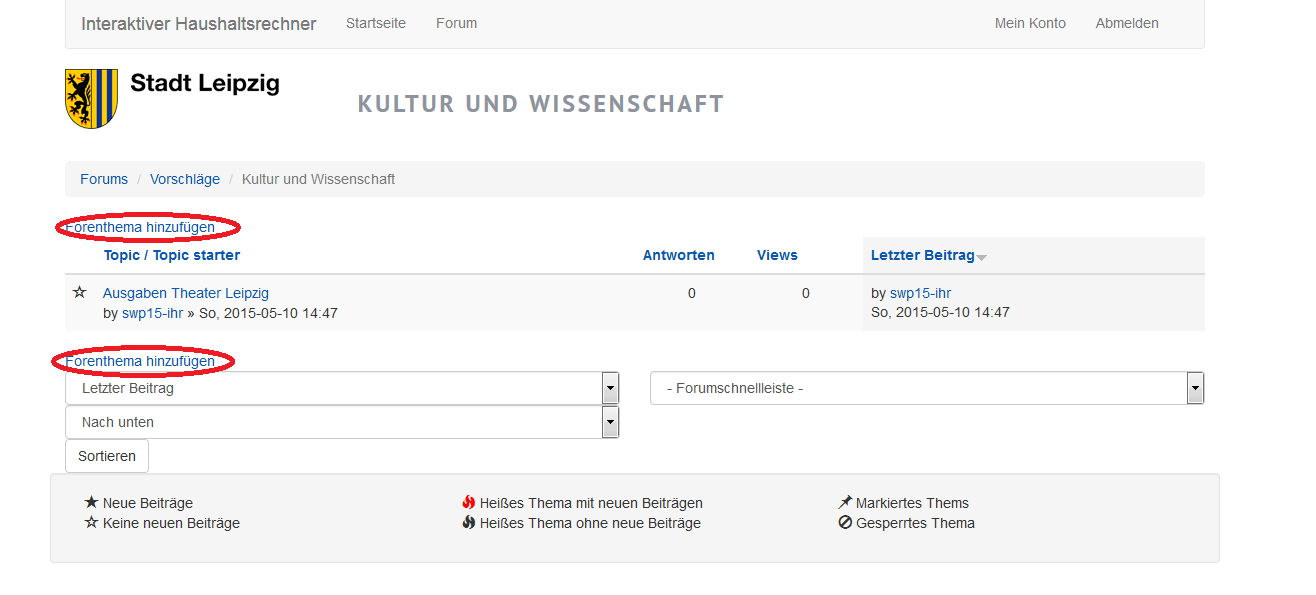
\includegraphics[width=\textwidth]{Bilder/forumtopic.png}
\end{center}

\subsection{Vorschl\"age sortieren und anschauen}
Sofern Sie auf einen Bereich gedr\"uckt haben, sehen Sie alle Vorschl\"age in
diesem Bereich mit jeweils Namen, Autor, Datum, Antworten, Anzahl der
Personen, die ihn sich angeschaut haben und dem Autor des letzten Kommentares.

\begin{center}
  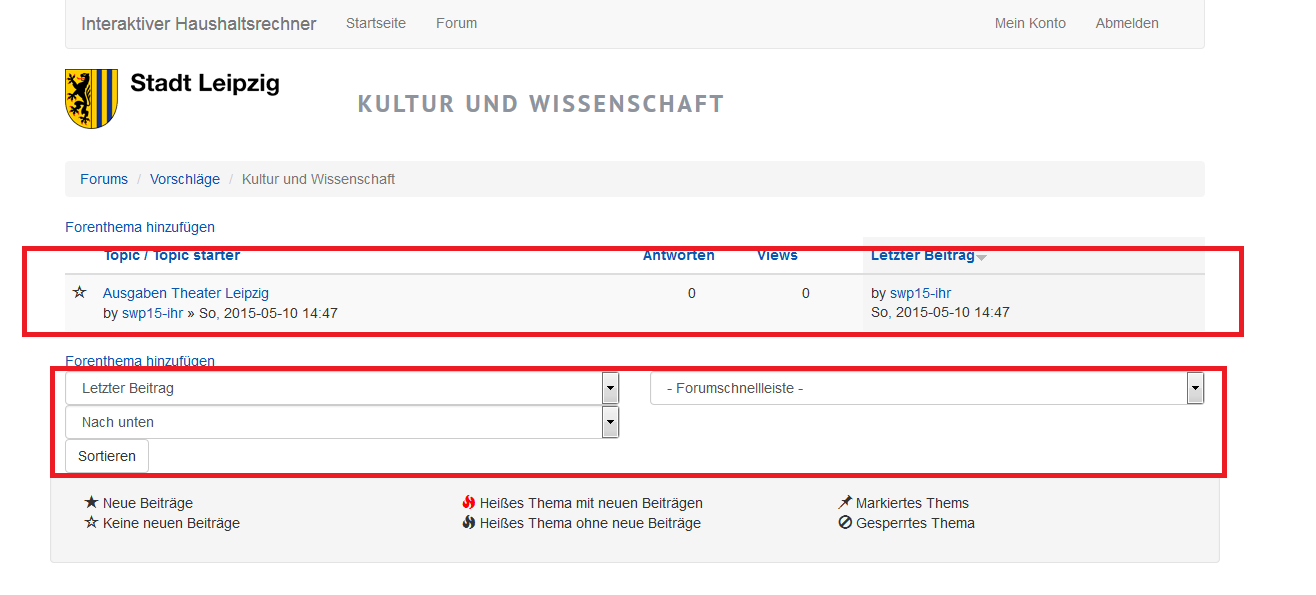
\includegraphics[width=\textwidth]{Bilder/forumsort.png}
\end{center}
Im unteren Bereich k\"onnen Sie die Beitr\"age nach gewissen Eigenschaften
sortieren. Sofern Sie ihre gewollte Auswahl getroffen haben, k\"onnen Sie auf
"`Sortieren"' dr\"ucken.

\subsection{Vorschl\"age kommentieren und bewerten}
Unter dem Text des Autors k\"onnen Sie durch dr\"ucken von + oder - eine
Bewertung abgeben, diese kann wieder ge\"andert werden durch dr\"ucken des
anderen Buttons.

\begin{center}
  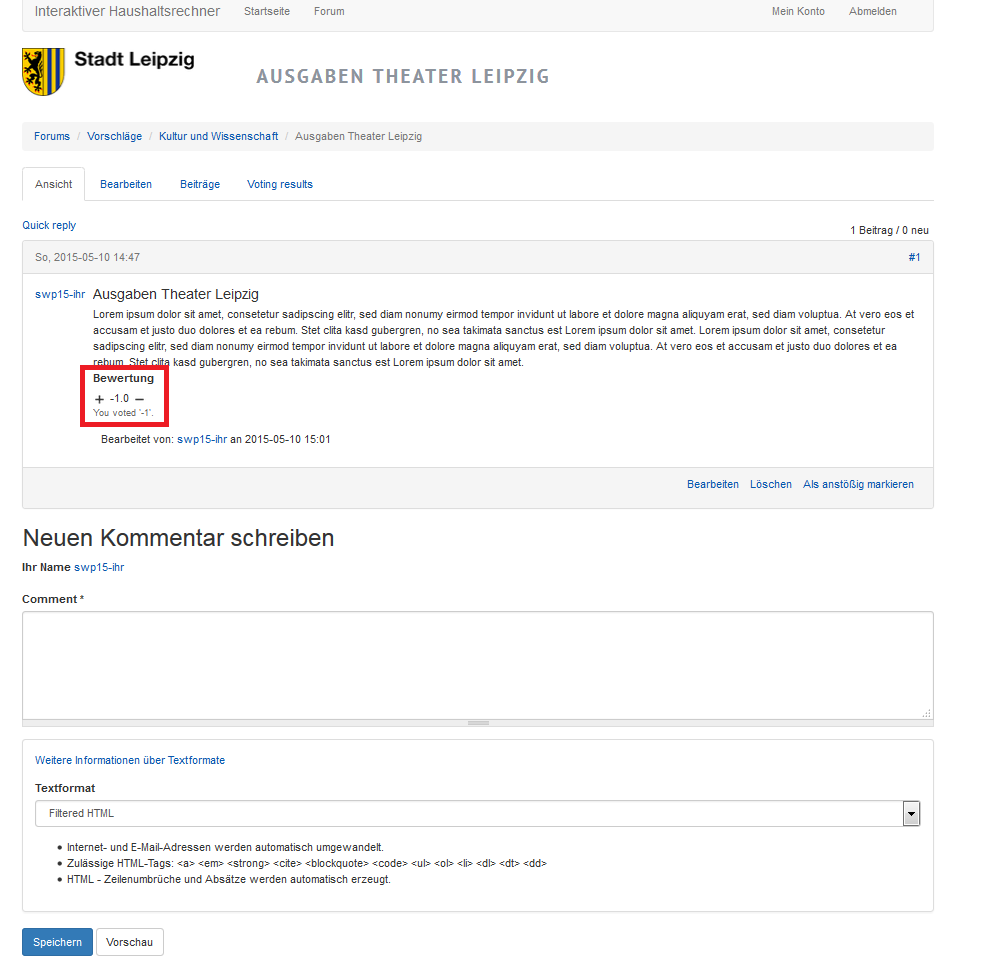
\includegraphics[width=\textwidth]{Bilder/comment.png}
\end{center}
Um einen Kommentar zu erstellen, schreiben Sie einfach ihr Kommentar in die
daf\"ur vorgesehene Box und dr\"ucken Sie auf Vorschau um zu sehen, wie Ihre
Nachricht aussehen w\"urde und speichern, um direkt zu kommentieren.
\end{document}
